\documentclass[12pt]{article}
\usepackage{ctex}
\usepackage[english]{babel}
\usepackage{blindtext}
\usepackage{nameref}
\usepackage{fancyhdr}
\usepackage{amsmath,amssymb,amsthm}
\usepackage{graphicx,float}
\usepackage{physics}
\usepackage{pgfplots}
\usepackage[a4paper, total={6in, 9in}]{geometry}

\graphicspath{{../images/}}

\pagestyle{fancy}
\fancyhf{}
\fancyhf[HL]{Circle challenge}
\fancyhf[HR]{}
\fancyhf[CF]{\thepage}

\newcommand{\innerprod}[2]{\langle{#1},{#2}\rangle}
\newcommand{\id}{\mathtt{id}}

\newtheorem*{definition}{Definition}
\newtheorem*{theorem}{Theorem}
\newtheorem*{corollary}{Corollary}
\newtheorem*{lemma}{Lemma}
\newtheorem*{proposition}{Proposition}
\newtheorem*{remark}{Remark}
\newtheorem*{claim}{Claim}
\newtheorem*{example}{Example}
\newtheorem*{axiom}{Axiom}

\begin{document}
    Using coordinate system to construct a circle, we find that if a circle is centered at $(h,k)$ with radius $r$, then by Pythagoras theorem (or distance formula), we have the following thought:

    Let $P$ be a moving point on the circumference of that circle, the distance between $P$ and the center of the circle is fixed by radius $r$. Therefore, the equation of the circle (in fact circumference) is given by the following equation: $$(x-h)^2+(y-k)^2=r^2$$

    By expansion and rearrangement of terms of the equation, we have the equation becomes $$x^2+y^2+Dx+Ex+F=0$$ where $D,E,F$ are real coefficients computed by $D=-2h, E=-2k, F=h^2+k^2-r^2$.

    Moreover, we call circles of the same center \textbf{concentric circles}.

    \subsection*{Challange}

    Given a circle $C_0:x^2+y^2=R^2$, where $R>0$. Let $P(h,k)$ be a moving point on $C_0$. We construct another circle $C_P$ centered at $P$ with radius $r$, where $0<r<R$. Let $F$ and $G$ be the closest point from the origin to $C_P$ and the farthest point from the origin to $C_P$ respectively. Denote the locus of $F$ and $G$ by $C_F$ and $C_G$ respectively.

    \begin{enumerate}
        \item Describe the geometric relationship between $O,F$ and $G$.
        \item Find the equation of straight line for $OP$ in terms of $h,k$ and $R$.
        \item Find the coordinates of $F$ and $G$ in terms of $h,k,R$ and $r$.
        \item Prove that $C_F$ and $C_G$ are concentric circles.
        \item Define the tangent lines of $C_P$ passing through the origin to be $L_1$ and $L_2$. Find the area enclosed by $L_1,L_2,C_F,C_G$ and $C_P$.
    \end{enumerate}

    \newpage

    \section*{Challenging problems set}

    \begin{enumerate}
        \item Let $\triangle ABC$ be with arbitrary sides $a,b,c$. Compute the ratio of area of the triangle to its inscribed circle. 
        \item Refer to the following diagram:
        \begin{figure}[H]
            \centering
            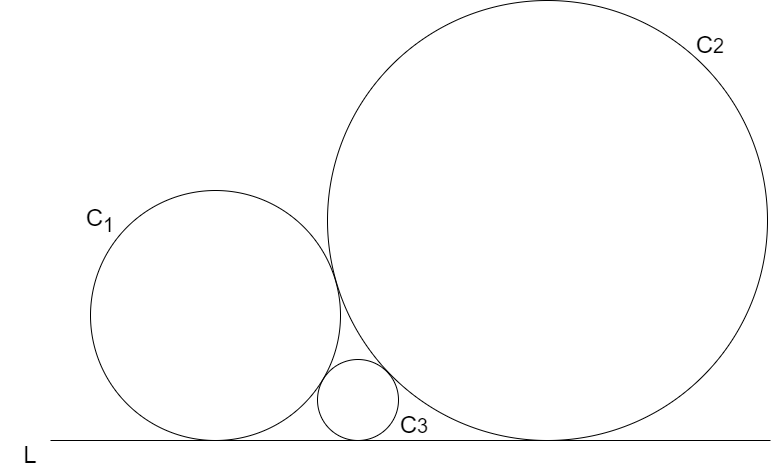
\includegraphics[scale=0.5]{cotangent_circles.png}
        \end{figure}
        Suppose as shown in the figure that three circles $C_1,C_2,C_3$ are all touching others at one point, and they share the same taangent line $L$. Denote the touching point of $C_1$ and $L$ be $X$, the touching point of $C_2$ and $L$ be $Y$, the touching point of $C_3$ and $L$ be $Z$, the touching point of $C_1$ and $C_2$ be $P$, the touching point of $C_1$ and $C_3$ be $Q$, the touching point of $C_2$ and $C_3$ be $R$. If $XZ=1$ and $YZ=2$, find the area of $\triangle PQR$. 
    \end{enumerate}
\end{document}